% ================================================================= 11
\section{Results on LongMemEval}\label{sec:lme}

\begin{table}[!htb]
\centering\small
\setlength{\tabcolsep}{4pt}
\begin{tabular}{@{}l c r r r r@{}}
\toprule
\thead{System} & \thead{Accuracy (95\% CI)} & \thead{vs mem0 (paired)} & \thead{Memory tokens} & \thead{Recall p50} & \thead{Evidence recall}\\
\midrule
\mx{} full memory & \best{89.0\%} [80, 94] & 12 / 2, $p=0.013$ & 24,464 & 631 ms & 0.99\\ \rowrule
\mx{} ranked (4k) & 80.5\% [71, 88] & 12 / 9, $p=0.66$ & \best{358} & 650 ms & 0.89\\ \rowrule
mem0 top-30 & 76.8\% [67, 85] & -- & 1,650 & 689 ms & 0.91\\ \rowrule
chunk RAG (4k) & 73.2\% [63, 82] & 11 / 14, $p=0.69$ & 3,968 & -- & 0.91\\ \rowrule
full context & 68.3\% [58, 77] & 10 / 17, $p=0.25$ & 117,009 & -- & \best{1.00}\\
\bottomrule
\end{tabular}
\caption{\textbf{LongMemEval-S, 82 questions.} \mx{} and mem0 ingested every history fresh with Haiku 5.5; all systems
answered with Haiku 4.5 and were judged by Sonnet 5.5. ``vs mem0'': questions only this system / only mem0 got right,
exact McNemar. Memory tokens: mean block given to the answering model. Evidence recall: share of gold evidence sessions
represented in that block.}
\label{tab:lme}
\end{table}

\begin{figure}[!htb]
\centering
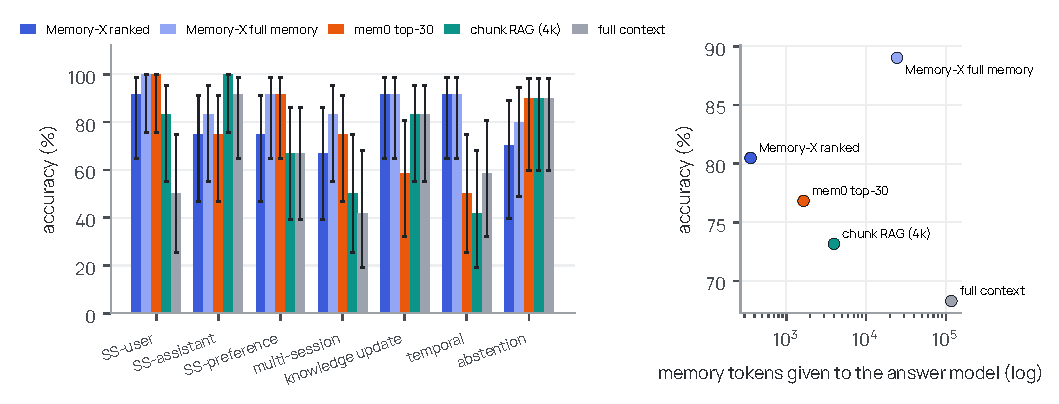
\includegraphics[width=\linewidth]{figures/fig_lme.pdf}
\caption{\textbf{Accuracy by question type} (left, Wilson 95\% intervals) and \textbf{against memory-block size}
(right, log scale).}
\label{fig:lme}
\end{figure}

\mx{} ranked recall answered 80.5\% of questions from a 358-token block, \textbf{4.6 times smaller} than mem0's 1,650
tokens, against mem0's 76.8\% (12 to 9, not significant). With its full memory \mx{} reached 89.0\%, significantly
above mem0 (12 to 2, $p=0.013$), chunk retrieval (17 to 4, $p=0.007$) and full context (20 to 3, $p<0.001$). The
largest per-type gaps are on temporal reasoning (11 of 12 against mem0's 6) and knowledge updates (11 against 7), where
\mx{}'s dated related facts and replaced-version history let the answering model pick the newer value. Ranked recall
keeps 1.5\% of the full memory's tokens; the gap to full memory (1 to 8, $p=0.04$) is spread across question types,
mostly facts the grader judged background that the answer needed.

\begin{figure}[!htb]
\centering
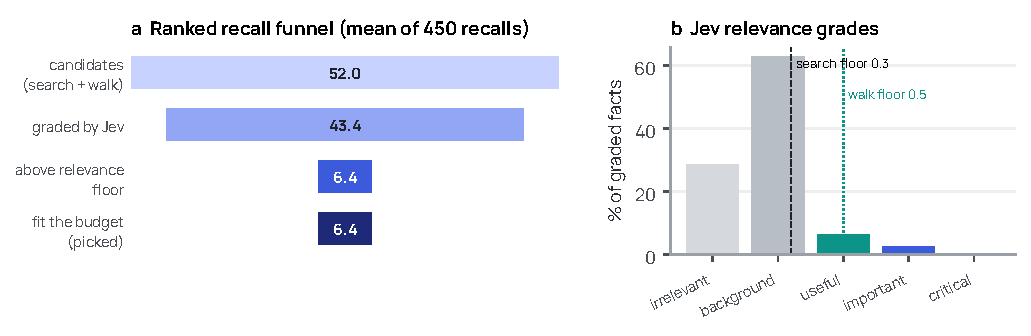
\includegraphics[width=\linewidth]{figures/fig_recall.pdf}
\caption{\textbf{What ranked recall does with its candidates} on LongMemEval. (a) Mean facts per step. (b) Jev's
relevance grade for every graded fact.}
\label{fig:recall}
\end{figure}

\paragraph{Where the small block comes from} One Jev request grades about 43 candidates per question; 90\% are graded
\emph{irrelevant} or \emph{background} and cut, leaving about 6 facts (Figure~\ref{fig:recall}).

\paragraph{Ingest cost} With the cost cuts of Section~\ref{sec:arch}, \mx{} ingest cost \$0.142 per history (extraction
\$0.055, Jev \$0.087) against about \$0.13 for mem0, storing 552 facts per history. Before the cuts the same histories
cost \$0.214 and produced 811 facts, with no loss of accuracy on a 10-question check (8 and 9 of 10 correct,
Table~\ref{tab:extractcost}).

\begin{table}[!htb]
\centering\small
\begin{tabular}{@{}l r r r r r@{}}
\toprule
\thead{Per history, Haiku 5.5} & \thead{Facts} & \thead{Output tokens} & \thead{Extraction} & \thead{Jev} & \thead{Total}\\
\midrule
before the cuts & 811 & 113k & \$0.100 & \$0.114 & \$0.214\\ \rowrule
after the cuts & \best{552} & \best{63k} & \best{\$0.055} & \best{\$0.087} & \best{\$0.142}\\ \rowrule
mem0 (reference) & & & & & \$0.13\\
\bottomrule
\end{tabular}
\caption{\textbf{Extraction cost.} The cuts: an assistant's list as one fact, a slimmer output schema, continuation
instead of re-extraction, a cached prompt prefix and the chit-chat gate. Measured from per-ingest receipts (cache reads at the cache-read price) and metered
Jev cost. The chit-chat gate rarely fires on LongMemEval (about one turn per history). Batch extraction for queued
inserts halves the extraction price again; it is not used in the benchmarks.}
\label{tab:extractcost}
\end{table}
